\DailyTitle{6272 Log (October 5, 2010)}

\DailySection{Goals}

\begin{enumerate}
\item Install DQM from Artur
\item Fit!
\item Finish up Hcal signal sample shape
\end{enumerate}

\DailySection{Summary List}

\begin{enumerate}
\item Hcal DQM basic code checkout.  The GUI is not installed yet.
\item Created signal pulse shape sample.
\item Compared signal and noise pulse shapes with the brainstorm ideas.
\item Met with Artur to briefly talk about noiseline ideas
\item Encorporated JP's isolation filter into the noiseline package
\item The float-all version of the candle fit works.
\end{enumerate}

\DailySection{Signal pulse shape for classification studies}

Comparing ADC collection might take a lot of time.  Changed to event number/run number.  The result looks fine from a test run.


\DailySection{Hcal DQM installation}

Following the instructions in the twiki page \url{https://twiki.cern.ch/twiki/bin/viewauth/CMS/HcalDQM},
I checked out the three packages in CMSSW version \texttt{3\_8\_2}.

\begin{verbatim}
cvs co -r V14-00-16      DQM/HcalMonitorClient
cvs co -r V14-00-10      DQM/HcalMonitorModule
cvs co -r V14-00-27      DQM/HcalMonitorTasks
scramv1 build
\end{verbatim}

Then proceed into running the test python configuration file.  The input file is missing but after relacing
the input list with a root file of \texttt{RAW} format, it runs fine.  The root file used is

\begin{verbatim}
/store/data/Run2010B/MinimumBias/RAW/v1/000/146/804/
   E89586EA-A0CA-DF11-BBD1-001617DBD472.root.
\end{verbatim}

After the job is done, there is a root file produced in the temp directory.  Inside there are a lot of root files
and pieces of information.  Does this mean that the installation was successful?

Now onto the GUI.  The twiki is at \url{https://twiki.cern.ch/twiki/bin/view/CMS/DQMTest}.

....Looks complicated.  Wait until Artur comes to see what is what.

\DailySection{Meeting with Artur on CMS noiseline}

We agreed on trying the following

\begin{enumerate}
\item Put in the noise filters (standard one, JP isolation filter) to the noiseline
\item Are there spike in $|i\eta|$ 85?
\item Double-spike algorithm
\item Try to run on the runs from last week where the bad channel is unmasked accidentally.  And see if it can be picked out.
\end{enumerate}

\DailySection{Adding basic filters to the noiseline}

Checked out the JP isolation filter and it compiled fine.  However, the boolean value that was used to be there is gone.
So I copied the boolean part from his code (earlier version) and merged it into the current version.  One can now run
the python configuration file and use the result from the reflagging.

\DailySection{Vecbos Z fitting}

Updated the fit script.  New things:

\begin{enumerate}
\item The confusing yield plot is not produced anymore.  Instead, a table (plot) is produced which includes the yields.
\item Initial guess of signal yields is estimated using the total number of events and slope 0.2.
\item No top level models that contain signal/background.  Each jet bin is a model by itself and included in the final pdf separately.  This is to simplify the final yield calculation.
\end{enumerate}

Note.  If the initial guess is too far from reality, the errors will go crazy.  Sometimes they will be incredibly small (1e-8 level), or more often they will be larger than the fitted yields.
Currently I fix only $\alpha_L$.  The result of fit for calojet (30 GeV) and PF jet (30 GeV) are shown in figure \ref{Figure_6272FitSummaryPlotFloatAllCalo} and \ref{Figure_6272FitSummaryPlotFloatAllPF}.

\begin{figure}
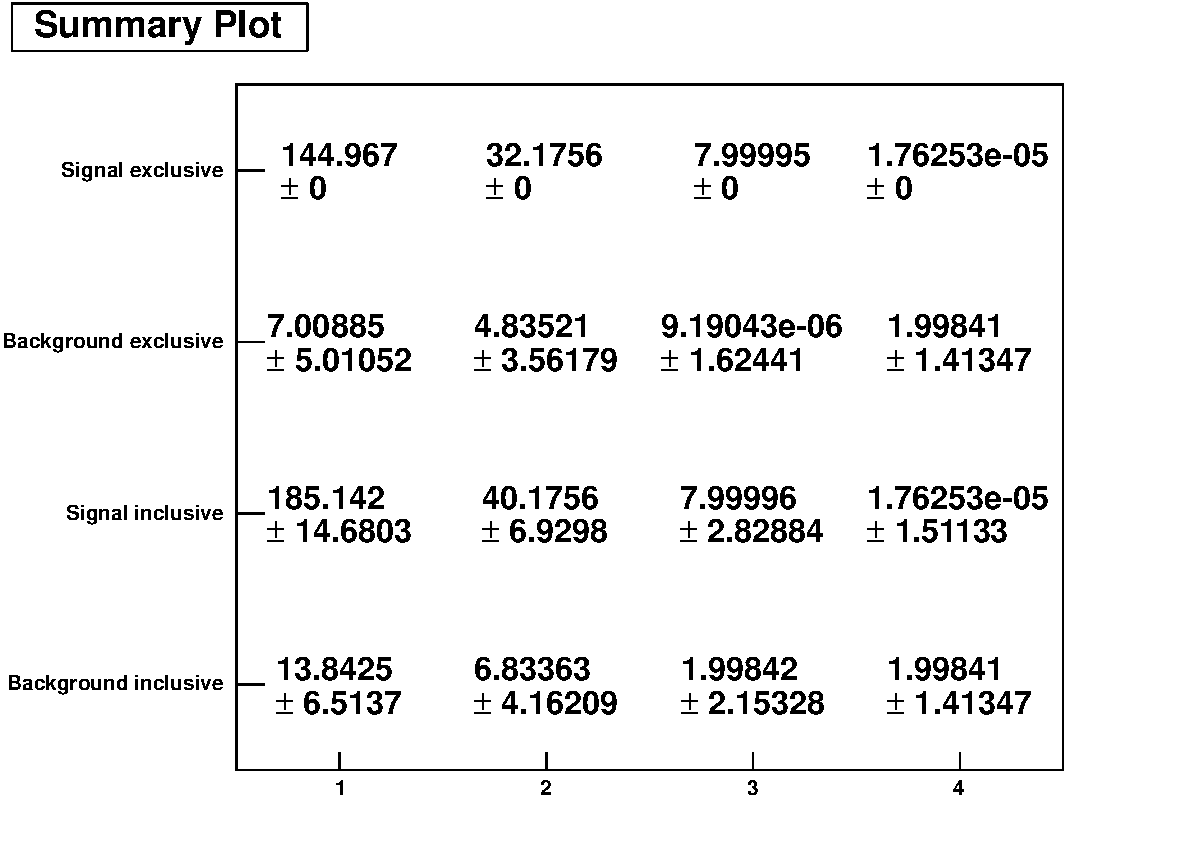
\includegraphics[width=120mm]{DailyLog/6272/6272_FitSummaryPlot_FloatAll_Calo}
\caption{Result of float-all-signal-yield fit of Calo jets with 30 GeV.  No restriction on relative yield is applied.  The error on inclusive yield is from roofit directly.  The fit takes care of the error.
The error on exclusive signal yield is not defined for \texttt{RooFormulaVar}, so it shows zero.  The out-of-the-box background yields are the exclusive ones, and the inclusive yield errors
are added in quadrature.  ($\alpha_L$ is fixed to 0.485)}
\label{Figure_6272FitSummaryPlotFloatAllCalo}
\end{figure}

\begin{figure}
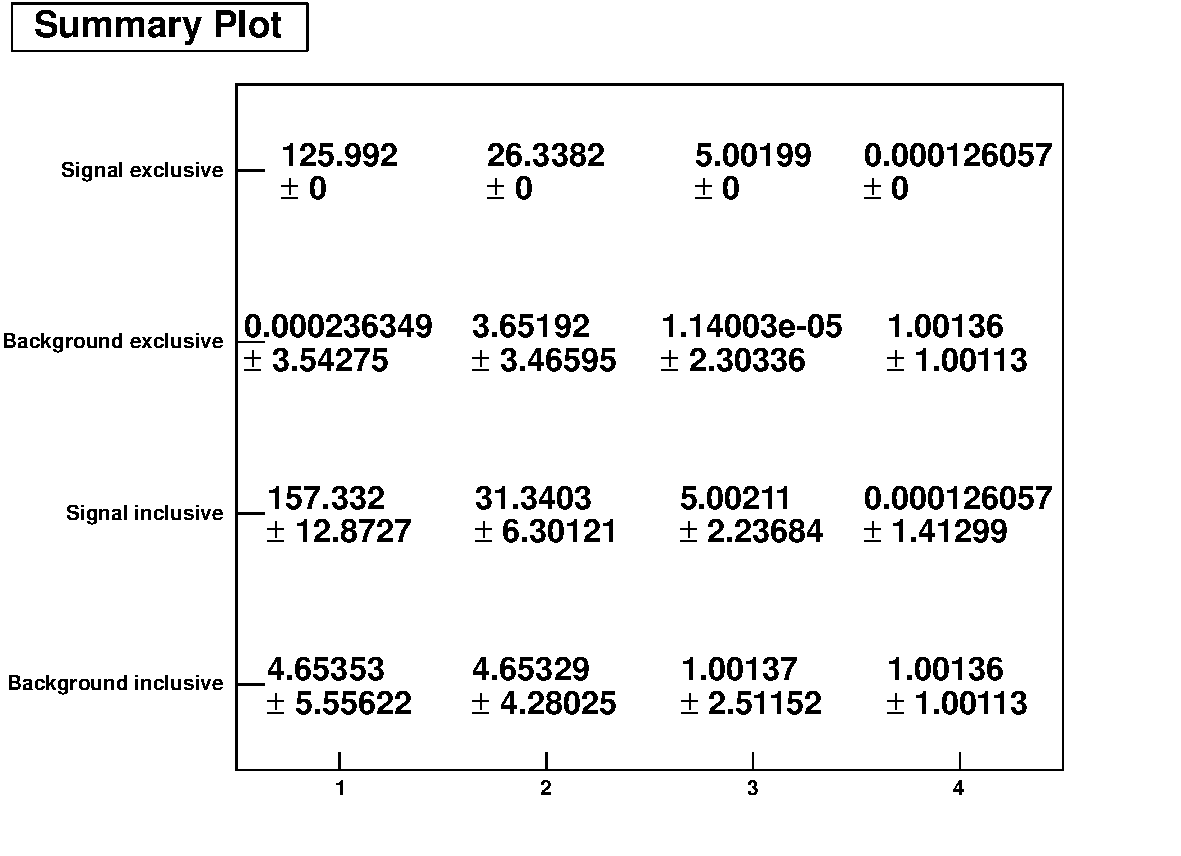
\includegraphics[width=120mm]{DailyLog/6272/6272_FitSummaryPlot_FloatAll_PF}
\caption{Result of float-all-signal-yield fit of PF jets (30 GeV).  Refer to the calojet one (figure \ref{Figure_6272FitSummaryPlotFloatAllCalo})
for more information.}
\label{Figure_6272FitSummaryPlotFloatAllPF}
\end{figure}

Description of the fit implemented.

\begin{enumerate}
\item Each jet bin is to have its own function.  Cruijff for signal, and exponential for background.  The function for each jet bin is multiplied by a \texttt{RooSameAs} or \texttt{RooAtLeast}
to constrain it in the designated bin.
\item The bins are exclusive, except the last one.
\item Signal yields are declared to be inclusive, and the number assigned to the signal function in each jet bin is a \texttt{RooFormulaVar} which is just the subtraction
of the two relavent inclusive numbers (except the last one).
\item Initial guess of inclusive signal yields is the total number of events, with slope 0.2.
\item The cruijff function is constrained to be exactly the same in all jet bins.
\item The $\alpha_L$ value is fixed, and all others are left floating.
\end{enumerate}

\DailySection{Reflection}

Not enough focus on vecbos....  The DQM work can be slower.


\DailySection{Goals for next work day}

\begin{enumerate}
\item Read and understand the double spike algorithm
\item Make sure if anyone is doing the vecbos PDMu dataset
\item Make a set of loose cuts to remove obvious noise, and skim through pulse shapes of the rest
\item Port the HCAL ideal pulse shape (as in \texttt{CMSSW}) to \texttt{RooFit}
\item Vecbos fitting strategy?
\item To-do chart for ZJets candle note for fast execution once target data ($\sim 50 pb^{-1}$) arrives
\end{enumerate}


